\documentclass[10pt]{beamer}
\usefonttheme{professionalfonts}
%\usetheme{Rochester}
%\usetheme{AnnArbor}
\usetheme{Szeged}
\useoutertheme{infolines}
\usecolortheme{dolphin}
\usepackage{graphicx}
% \usepackage[english]{babel}
\usepackage{hyperref}
\usepackage{multicol}
\usepackage{color}
%\usepackage{smartdiagram}


%\definecolor{carmine}{rgb}{0.59, 0.0, 0.09}
\usepackage{amsmath} 

\usepackage{graphicx}
\usepackage{tikz}
\usetikzlibrary{shapes.callouts}
\usepackage{multirow}

\usepackage[utf8]{inputenc}

\usepackage{enumerate}
\usepackage[shortlabels]{enumitem}
\usepackage{amsmath,amsthm,amssymb,amsfonts,mathrsfs,latexsym,stmaryrd}
\usepackage{tcolorbox}

\usepackage{color} 
\usepackage{amssymb, amsmath, amsbsy}
\usepackage{adjustbox,lipsum}
\usepackage{placeins}

\usepackage{textpos}
\usepackage{wrapfig}
\usepackage[spanish, es-tabla]{babel}

\usepackage{caption}
\setlength{\parindent}{15pt}
%\usepackage[hyperfootnotes=false]{hyperref}

\usepackage{url}
\usepackage{float}
\usepackage{tikz}
\usetikzlibrary{patterns}


\title[ICS-294]{Econometría ICS-294\\ \small{Clase 5: Error de medición}}

\author{Francisco Alfaro Medina}
\institute[USM]
{Universidad Técnica Federico Santa María\\ % Your institution for the title page
	\medskip
	\textit{} % Your email address
	
}
\logo{

\includegraphics[width=1cm]{../Imagenes/Logo_UTFSM.png}
}
\date{}
\newcommand\Fontvi{\fontsize{9}{7.2}\selectfont}
\begin{document}
	
\begin{frame}
	\titlepage % Print the title page as the first slide
\end{frame}

\section{Error de Medición}

\begin{frame}{El mundo real}
    \begin{itemize}
       
        \item Cuando tratamos de estimar la relación entre variables, hay que usar lo que está disponible en los datos reales. 
        \item A menudo, no se cuenta con datos sobre la variable económica que realmente nos interesa.
        \item Ejemplo
        \begin{itemize}
            \item Ingreso verdadero vs. ingreso declarado
            \item Calor\'ias consumidas vs. calor\'ias compradas
        \end{itemize}
        
    \end{itemize}
\end{frame}

\begin{frame}{Error de Medición}
    \begin{itemize}
        \item La variable que nos interesa es $W^{*}$, pero solo tenemos una versión imprecisa de esta variable donde:
$$
W=W^{*}+u
$$
\item Se define como ``error de medida" $u=W-W^{*}$. Es decir, la diferencia entre la variable que observamos y la verdadera variable.
\item Supongamos el error menos grave posible. Lo llamamos error cl\'asico cuando $E(u)=0$ y $\operatorname{Cov}(u, W^{*})=0$.
\item ¿Qué pasa si tenemos errores de medición cl\'asico en la variable dependiente? ¿E independiente?
    \end{itemize}
\end{frame}

\section{Error de medición en la variable dependiente}

\begin{frame}{Error de medición en la variable dependiente}
    \begin{itemize}
        \item Considere el siguiente modelo verdadero,  no hay sesgo por variable omitida: 

        \begin{eqnarray}
                                   Y^{*}=\beta_{0}+\beta_{1} X+\varepsilon\\
                                   E[\varepsilon \mid X]=0  \nonumber
       \end{eqnarray}
        \item Pero en lugar de $Y^{*}$ solamente tenemos $Y=Y^{*}+u$. Donde el error de medici\'on lo asumimos cl\'asico: $\operatorname{Cov}\left(Y^{*}, u\right)=0$ y $V(u)=\sigma_{u}^{2}$.
        \item Si sustituimos $Y-u=Y^{*}$ en (1) y despejamos, podemos estimar:
            
        \begin{equation}
             Y=\beta_{0}+\beta_{1} X+v        \end{equation}
       
        
        \item Donde $v=(\varepsilon+u)$
        \item ¿Ser\'a $\hat{\beta}_{1}$ insesgado?
        \item Como suponemos que el error de medici\'on de la variable $Y$ {\color{blue} no} esta correlacionado con X, entonces no causar\'a sesgo.
    \end{itemize}
\end{frame}

\begin{frame}{Error de medición en la variable dependiente}
    \begin{itemize}
              \item Para que los estimadores $\hat{\beta}_{0}$ y $\hat{\beta}_{1}$ sean insesgados, necesitamos que
        $$
        E\left(\hat{\beta}_{1}\right)=\beta_{1}
        $$
        \item Sabemos que
        $$
        \begin{gathered}
        E\left(\hat{\beta}_{1}\right)=\frac{\operatorname{Cov}(X, Y)}{\operatorname{Var}(X)}=\frac{\operatorname{Cov}\left(X, Y^{*}+u\right)}{\operatorname{Var}(X)} \\
        E\left(\hat{\beta}_{1}\right)=\frac{\operatorname{Cov}\left(X, Y^{*}\right)}{\operatorname{Var}(X)}+\frac{\operatorname{Cov}(X, u)}{\operatorname{Var}(X)} \\
        E\left(\hat{\beta}_{1}\right)=\beta_{1}
        \end{gathered}
        $$
        \item {\color{blue}Dado que $\operatorname{Cov}(X, u)=0$ por la definición del error clásico.}
    \end{itemize}
\end{frame}

\begin{frame}{Intuición}
    Si el error de medida en la variable dependiente no está sistemáticamente relacionado con las variables explicativas, entonces el estimador MCO sigue siendo insesgado.
\end{frame}
\begin{frame}{Impacto sobre precisión}
    \begin{itemize}
        \item  Sin embargo, los estimadores de MCO van a tener mayores varianza
       
        
        \item Con errores de medición en la variable dependiente, el t\'ermino del error es $\varepsilon+u$. Y entonces, su varianza es $\operatorname{Var}(\varepsilon)+\operatorname{Var}(u)>\operatorname{Var}(\varepsilon)$.
    \end{itemize}
\end{frame}

\section{Errores de medición en variables independientes}

\begin{frame}{Ejemplo: Relación entre salario e IQ}
    \begin{figure}
        \centering
        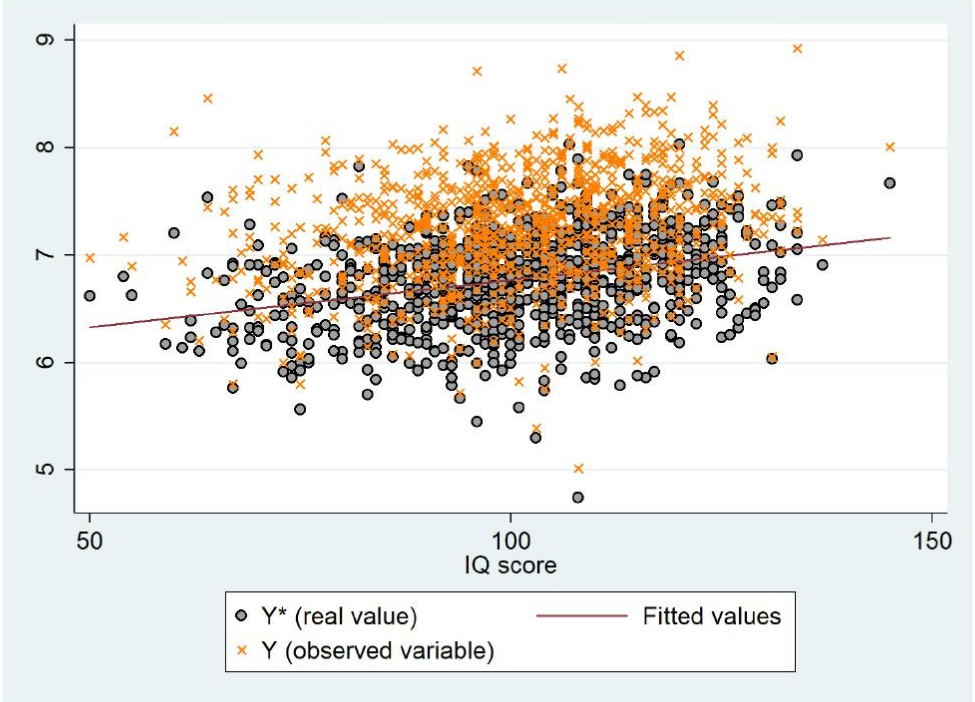
\includegraphics[width=0.75\linewidth]{../Imagenes/RelacionSalarioIQ.jpeg}
    \end{figure}
\end{frame}

\begin{frame}{Errores de medición en variables independientes}
    \begin{itemize}
        \item Cuando la variable mal medida es la independiente, el problema es m\'as grave.
        \item La variable que nos interesa es $X^{*}$, pero solo tenemos una versión imprecisa de esta variable donde
        $$
        X=X^{*}+u
        $$
        \item Vamos a seguir suponiendo errores clásicos, es decir que $\operatorname{Cov}\left(X^{*}, u\right)=0$ y $V(u)=\sigma_{u}^{2}$.
    \end{itemize}
\end{frame}

\begin{frame}{Impacto sobre MCO}
    \begin{itemize}
        \item El modelo verdadero es:
        \begin{equation*}
        Y=\beta_{0}+\beta_{1} X^{*}+\epsilon \tag{1}
        \end{equation*}
        \item Donde asumimos que $E\left[\epsilon \mid X^{*}\right]=0$
        \item Pero podemos estimar:
        \begin{equation*}
            Y=b_{0}+b_{1} X+v \tag{2}
        \end{equation*}

        \item $v=\epsilon-\beta_1u$
        \item Vamos a ver que ahora el estimador $\hat{b}_1$ va a ser sesgado.
    \end{itemize}
\end{frame}

\begin{frame}{Sesgo de atenuaci\'on - sesgo por error de medici\'on en X}
    \begin{itemize}
        \item Estimamos:
        $$
        \begin{gathered}
        Y=b_{0}+b_{1} X+v \\
        E\left[\hat{b}_{1}\right]=\frac{\operatorname{Cov}(X, Y)}{\operatorname{Var}(X)}=\frac{\operatorname{Cov}\left(X^{*}+u, Y\right)}{\operatorname{Var}\left(X^{*}+u\right)}
        \end{gathered}
        $$
        \item Dado que el error es clásico: $\operatorname{Cov}(u, Y)=0$ por lo que:
        $$
        E\left[\hat{b}_{1}\right]=\frac{\operatorname{Cov}\left(X^{*}, Y\right)}{\operatorname{Var}\left(X^{*}+u\right)}
        $$
        \item Además, el denominador lo podemos escribir como la suma de varianzas:
        $$
        \operatorname{Var}\left(X^{*}+u\right)=\operatorname{Var}\left(X^{*}\right)+\operatorname{Var}(u)
        $$
        \item Reemplazando $Y$ por el modelo original (1):
        $$
        E\left[\hat{b}_{1}\right]=\frac{\operatorname{Cov}\left(X^{*}, \beta_{0}+\beta_{1} X^{*}+\epsilon\right)}{\operatorname{Var}\left(X^{*}\right)+\operatorname{Var}(u)}
        $$
    \end{itemize}
\end{frame}

\begin{frame}
    \begin{itemize}
        \item separando las covarianzas:
        $$
        E\left[\hat{b}_{1}\right]=\frac{\beta_{1} \operatorname{Cov}\left(X^{*}, X^{*}\right)+\operatorname{Cov}\left(X^{*}, \epsilon\right)}{\operatorname{Var}\left(X^{*}\right)+\operatorname{Var}(u)}
        $$
        \item Sabemos que el modelo real esta bien especificado por lo que $\operatorname{Cov}\left(X^{*}, \epsilon\right)=0$. Ademas, por definici\'on, $\operatorname{Cov}\left(X^{*}, X^{*}\right)=\operatorname{Var}\left(X^{*}\right)$.
        \item Entonces:
        $$
        E\left(\hat{b}_{1}\right)=\beta_{1} \frac{\operatorname{Var}\left(X^{*}\right)}{\operatorname{Var}\left(X^{*}\right)+\operatorname{Var}(u)}=a \cdot \beta_{1}
        $$
        \item Noten que $a<1$.
        \item Por eso se llama sesgo de atenuaci\'on. El coeficiente de MCO ser\'a m\'as pequeño en valor absoluto, subestimaremos el efecto.
    \end{itemize}
\end{frame}

\begin{frame}{Sesgo de atenuación}
    $$
    E\left(\hat{b}_{1}\right)=\beta_{1} \frac{\operatorname{Var}\left(X^{*}\right)}{\operatorname{Var}\left(X^{*}\right)+\operatorname{Var}(u)}=a \cdot\beta_{1}
    $$
    \begin{itemize}
        \item Si $\beta_{1}>0$, el estimador será menor al par\'ametro.
        \item Si $\beta_{1}<0$, el estimador será mayor al par\'ametro, menor en valor absoluto.
        \item Entonces, tenderemos a subestimar (en valor absoluto) la magnitud de la pendiente.
        \item La magnitud del sesgo depende de cuan grande es $\operatorname{Var}(u)$ comparado a $\operatorname{Var}(X)$. Esto se llama: "signal-to-noise ratio".
    \end{itemize}
\end{frame}

\begin{frame}{Ejemplo simple: horas de estudio y nota}
    \begin{itemize}
        \item Supongamos que el modelo verdadero es:
        $$
        Nota=\beta_{0}+2\cdot Horas^{*}+\epsilon
        $$
        \item Es decir, una hora adicional de estudio real aumenta la nota esperada en 2 puntos.
        \item Pero no observamos las horas reales $Horas^{*}$, sino un reporte con error:
        $$
        Horas=Horas^{*}+u
        $$
        \item Supongamos que:
        $$
        \operatorname{Var}(Horas^{*})=8 \quad \text{y} \quad \operatorname{Var}(u)=2
        $$
    \end{itemize}
\end{frame}

\begin{frame}{Ejemplo simple: sesgo de atenuaci\'on}
    \begin{itemize}
        \item Si estimamos usando $Horas$ en lugar de $Horas^{*}$:
        $$
        E\left(\hat{b}_{1}\right)
        =
        2\cdot
        \frac{8}{8+2}
        =
        1.6
        $$
        \item Aunque el efecto verdadero es $\beta_{1}=2$, MCO estima en promedio una pendiente menor.
        \item Intuici\'on: el ruido en $Horas$ aumenta la variabilidad de la variable explicativa, pero no agrega informaci\'on sobre $Nota$.
        \item Por eso el coeficiente se ``achica'' hacia cero.
    \end{itemize}
\end{frame}

\begin{frame}{Conclusiones}
    \begin{itemize}
        \item Cuando trabajamos con datos reales, no siempre medimos exactamente lo que queremos en nuestro modelo.
        \item Errores de medición de la variable dependiente no generan sesgo pero si aumentan varianza, dificultando el reconocimiento de relaciones entre variables.
        \item El error de medición en variables independientes genera sesgo de atenuación: siempre vamos a subestimar la magnitud de la relación entre variables.
    \end{itemize}
\end{frame}

\end{document}
